% !TEX TS-program = XeLaTeX
% !TEX encoding = UTF-8 Unicode

\documentclass[12pt]{article}

%\usepackage[utf8]{inputenc}
\usepackage[brazilian]{babel}

\usepackage{fontspec}
\setmainfont{Linux Libertine G}
\linespread{1.05}

%%% PAGE DIMENSIONS
\usepackage{geometry} % to change the page dimensions
\geometry{a4paper} % or letterpaper (US) or a5paper or....
% \geometry{margin=2in} % for example, change the margins to 2 inches all round
% \geometry{landscape} % set up the page for landscape

\usepackage{graphicx} % support the \includegraphics command and options

% \usepackage[parfill]{parskip} % Activate to begin paragraphs with an empty line rather than an indent

%%% PACKAGES
\usepackage{amsfonts}
\usepackage{color}
%\usepackage{booktabs} % for much better looking tables
%\usepackage{array} % for better arrays (eg matrices) in maths
%\usepackage{paralist} % very flexible & customisable lists (eg. enumerate/itemize, etc.)
\usepackage{verbatim} % adds environment for commenting out blocks of text & for better verbatim
\usepackage{microtype}
%\usepackage{subfig} % make it possible to include more than one captioned figure/table in a single float
% These packages are all incorporated in the memoir class to one degree or another...

\usepackage[hidelinks]{hyperref}

% For Computer Modern:
%\def\Cpp{{C\nolinebreak[4]\hspace{-.05em}\raisebox{.4ex}{\tiny\bf ++}}}
% For Linux Libertine G
\def\Cpp{{C\nolinebreak[4]\raisebox{.20ex}{\small\bf++}}}

\newcommand{\todo}[1]{\textsf{\color{red}#1}}

%%% END Article customizations

\title{Paralelização do compilador da linguagem de programação Rust}
\author{Yuri Kunde Schlesner}
%\date{} % Activate to display a given date or no date (if empty), otherwise the current date is printed 

\begin{document}
\maketitle

\section{Identificação}

\begin{description}
	\item[Resumo:] \todo{TODO.}
	\item[Período de execução:] Setembro de 2014 a Dezembro de 2014
	\item[Unidades participantes:] ~\\ Curso de Ciência da Computação \\ Departamento de Eletrônica e Computação
	\item[Área de conhecimento:] Ciência da Computação
	\item[Linha de Pesquisa:] Computação Gráfica, Linguagens de Programação
	\item[Tipo de projeto:] Trabalho de Conclusão de Curso
	\item[Participantes:] ~\\ Profª Andrea Schwertner Charão -- Orientadora \\ Yuri Kunde Schlesner -- Orientando
\end{description}

\section{Introdução}

A \emph{Computação Gráfica} é a area da Ciencia da Computação que estuda tópicos relacionados a criação, análise e manipulação de imagens e conceitos relacionados. Dentre estas, a síntese (ou renderização) de imagens é onde uma imagem é criada de forma computacional, a partir de um modelo matemático e frequentemente buscando o fotorealismo. Tem uma vasta quantidade de aplicações práticas: É usada na engenharia, durante o projeto de máquinas ou construções; na arquitetura para a visualização de espaços antes que sejam construídos; para entretenimento, em efeitos especiais de filmes ou em jogos 3D e em muitas outras aplicações.

Como a geração de imagens fotorealistas involve essencialmente uma simulação completa da física da luz, um processo proibitivamente lento e complexo, são utilizadas simplificações e modelos. No passado, devido a limitada capacidade computacional disponível, eram utilizadas aproximações grosseiras que, enquanto produziam imagens atrativas, não eram muito realísticas, especialmente no quesito da aparência das superfícies de suas interações com a luz. Com o aumento do poder computacional disponível, vem sendo usados modelos cada vez mais fiéis a realidade e que produzem imagens cada vez mais convincentes, algumas vezes indistinguíveis de uma fotografia real.

\emph{Path tracing} é um método de renderização que assume que a luz se comporta como uma partícula e calcula uma imagem traçando uma série de raios pelos caminhos através quais a luz viajaria quando refletida através de uma cena. Atualmente é um dos algorítmos mais usados quando são demandadas imagens com um grau de realismo extremamente alto, devido a sua abilidade de simular o comportamento da luz com relativa precisão.

No entanto, este realismo vem ao custo de muito poder de processamento, e mesmo com o avanço tecnológico de CPUs, a renderização de imagens continua sendo uma das tarefas mais árduas para processadores. Sistemas de renderização profissionais são quase exclusivamente escritos em \Cpp, e não em linguagens de mais alto nível, devído as penalidades de performance que impõem, e sistemas mais recentes chegam a fazer o uso de GPUs para acelerar a imensa quantidade de cálculos necessária. Tendo em vista a baixa expressividade de \Cpp comparada a estas outras linguagens, torna-se interessante explorar alternativas que permitam mais fácil desenvolvimento, mas sem sacrificar a performance requerida.

A linguagem de programação \emph{Rust}, um projeto de pesquisa da \emph{Mozilla Research}, tem como seu objetivo ser uma união entre linguagens de programação de sistemas e as tidas como ``linguagens de alto-nível'', focando simultâneamente em alta-performance, segurança e expressividade. Ela atinge isso usando um modelo tradicional de compilação prévia (\emph{ahead of time}) e um sistema de tipos que permite a verificação automática dos usos de ponteiros durante a compilação, eliminando a possibilidade de acontecerem erros de memória, mas sem introduzir penalidades excessivas de performance ou consumo de memória, ao mesmo tempo que integra conceitos mais recentes de linguagens de programação que aumentam sua expressividade e capacidade de facilmente descrever programas complexos.

\section{Objetivos}

\subsection{Objetivo Geral}

O objetivo geral deste trabalho é escrever um \emph{path tracer} simples em Rust que sirva de um exemplo educativo, juntamente com a fundamentação matemática que será descrita no relatório, de como implementar este tipo de algorítmo. Além disto, será uma oportunidade de fazer uma comparação qualitativa e quantitativa entre esta lingaugem e \Cpp, nos aspectos de performance e organização de código.

\subsection{Objetivos Específicos}
\begin{itemize}
	\item Re-escrever um renderizador (atualmente escrito em \Cpp) utilizando a linguagem Rust.
	\item Realizar uma comparação de performance e clareza de código entre as duas versões.
	\item Implementar melhoras estruturais e algorítmicas na nova versão.
	\item Documentar a fundamentação teórica dos algorítmos utilizados.
	\item Analisar como as funcionalidades de Rust ajudam ou não a escrever um programa deste tipo.
\end{itemize}

\section{Justificativa}

Rust é uma linguagem relativamente nova e, embora aplicações gráficas de alta performance sejam um dos seus públicos alvo, ainda não existe uma quantidade significativa de programas deste tipo que valide a lingaugem para este propósito. A experiência e resultados adquiridos durante a realização deste trabalho podem ajudar a guiar o desenvolvimento da linguagem para atingir este fim.

Além disto, embora existam uma variadade de renderizadores pequenos que tem como objetivo servir de exemplo para outras implementações, eles no geral não possuem uma documentação adequada que explique os princípios teóricos e matemáticos por trás deles. Espera-se que este trabalho preencha este nicho, afim de ajudar futuros pesquisadores ou estudantes em busca deste conhecimento.

\section{Revisão de Literatura}

\todo{TODO.}

\begin{figure}
	\centering
	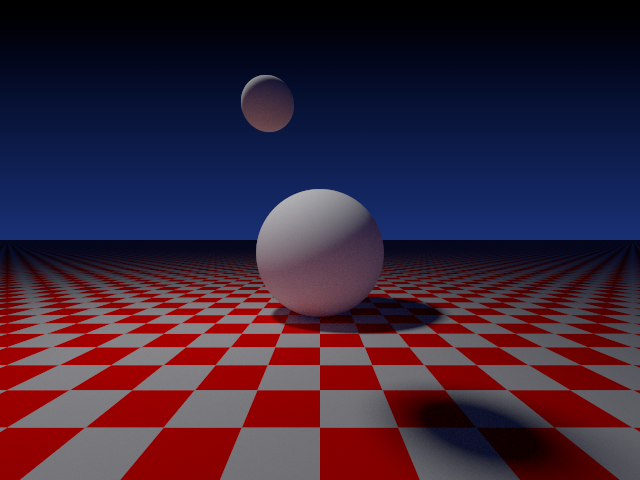
\includegraphics[width=0.5\textwidth]{exemplo_imagem}
	\caption{Um exemplo de uma imagem gerada utilizando \emph{path tracing}. Note como a luz que atinge o plano xadrez é refletida devolta para iluminar a esfera, um fenômeno conhecido como \emph{iluminação indireta} e que é corretamente simulado pelo algoritmo. \todo{(referenciar)}}
\end{figure}

\section{Metodologia}

Como tem como objetivo principal produzir uma síntese do conhecimento da área esta pesquisa tem um objetivo exploratório\todo{(descritivo?)}, e como irá produzir um trabalho que, além de guiar esta exploração, exemplificará a aplicação deste conhecimento, é também aplicada.

\section{Plano de Atividades e Cronograma}

\begin{enumerate}
	\item \label{activity:rewrite} \textbf{Re-escrever o renderizador utilizando a linguagem Rust:} O renderizador será baseado em código pré-existente do autor, escrito em \Cpp, que será utilizado como uma base funcional para a implementação em Rust.
	\item \label{activity:compare} \textbf{Realizar uma comparação entre as duas versões:} As duas versões do renderizador, a nova feita em Rust e a antiga em \Cpp, serão comparadas nos quesitos de performance e de organização do código, afim de identificar avanços ou regressos, e se esses podem ser atribuídos a características de cada linguagem.
	\item \label{activity:improve} \textbf{Implementar melhoras estruturais e algorítmicas:} A partir daqui, a nova versão do renderizador será aprimorada com algoritmos mais avançados, que permitam uma melhora de performance ou de qualidade de imagem. A maior parte do trabalho aqui será a revisão da bibliografia existente para identificar algorítmos interessantes e entender seu funcionamento.
	\item \label{activity:document} \textbf{Documentar a fundamentação teórica dos algorítmos:} Com a experiência adquirida durante a implementação, as observações e conclusões do autor serão sintetizadas com o objetivo de tornar claro o funcionamento destes algorítmos e como eles interagem.
	\item \label{activity:analysis} \textbf{Analisar como as funcionalidades de Rust ajudam ou não a escrever um programa desse tipo:} Continuando o trabalho da etapa \ref{activity:compare}, serão ressaltadas quaisquers constatações feitas durante o desenvolvimento sobre as vantagens ou desvantagens de se utilizar a Rust para este tipo de trabalho.
\end{enumerate}

Espera-se que o desenvolvimento das atividades siga o seguinte cronograma:

\begin{table}[h]
\centering
\begin{tabular}{c|cccc}
	Etapa & Setembro & Outubro & Novembro & Dezembro \\ \hline
	\ref{activity:rewrite} & \checkmark & & & \\
	\ref{activity:compare} & \checkmark & & & \\
	\ref{activity:improve} & & \checkmark & \checkmark & \\
	\ref{activity:document} & \checkmark & \checkmark & \checkmark & \checkmark \\
	\ref{activity:analysis} & & & & \checkmark \\
\end{tabular}
\caption{Cronograma de Atividades}
\end{table}

\section{Recursos}

Para a realização deste trabalho será utilizado apenas equipamento pessoal do pesquisador, visto que não é necessário o uso de qualquer equipamento especial além de um computador para desenvolvimento.

\section{Resultados Esperados}

Ao término deste trabalho, espera-se ter uma implementação de um renderizador, escrito em Rust, que seja capaz de produzir imagens fotorealísticas através da implementação de uma variedade de técnicas relacionadas a \emph{path tracing}. Além disso, espera-se que o relatório do trabalho sirva como uma síntese da teoria e funcionamento dos algorítmos implementados, de forma a guiar implementações futuras.

\section{Referências}

\todo{TODO.}

\end{document}
